\section{Binning of the \pth spectrum}
%%%%%%%%%%%%%%%%%%%%%%%%%%%%%%%%%%%%%%%%%%%%%%%%%%%%%%%%%%%%%%%%%%%%%%
\label{sec:Binning}

Given the limited resolution on $\pth$, a criterion is needed to establish bi size. The criterion that we have chose is devised to keep under control the bin migrations due to the finite resolution. 
For any given bin $i$ we can define the purity $P_i$ on a signal sample as the number events that are generated and also reconstructed in that bin, $N_i^{GEN|RECO}$, divided by the number of events reconstructed there $N_i^{RECO}$:
\begin{equation}
P_i = \frac{N_i^{GEN|RECO}}{N_i^{RECO}} \qquad .
\end{equation}
Where $N_i^{GEN|RECO}$ is the number of events that are both generated and
reconstructed in a $\pth$ bin $i$, while $N_i^{RECO}$ is the number of events
that are reconstructed in bin $i$. We have chosen the bin width in such a way
as to make the smallest bins able to ensure a purity of about 60\% on a gluon fusion sample.
Following this prescription we have divided the whole $\pth$ range in six
different bins: \mbox{[0-15 GeV]}, \mbox{[15-45 GeV]}, \mbox{[45-85 GeV]},
\mbox{[85-125 GeV]}, \mbox{[125-165 GeV]}, \mbox{[165-$\infty$ GeV]}.
%Mettere plot binning
A two-dimensional histogram  has been made putting the GEN level $\pth$ on the x-axis (calculated using the WW system transverse momentum) and the RECO one on the y-axis. Each row is then normalized to one in order to directly have the purity in the diagonal bins. Also the effect of bin migration due to finite detector resolution effects can be assessed from this plot.\\
This two dimensional plot is shown in Fig.~\ref{fig:response_by_row} (a) and (b) for gluon fusion and VBF signals for $m_\mathrm{H}=125$\GeV.
\begin{figure}[b]
\centering
\subfigure[ggH]{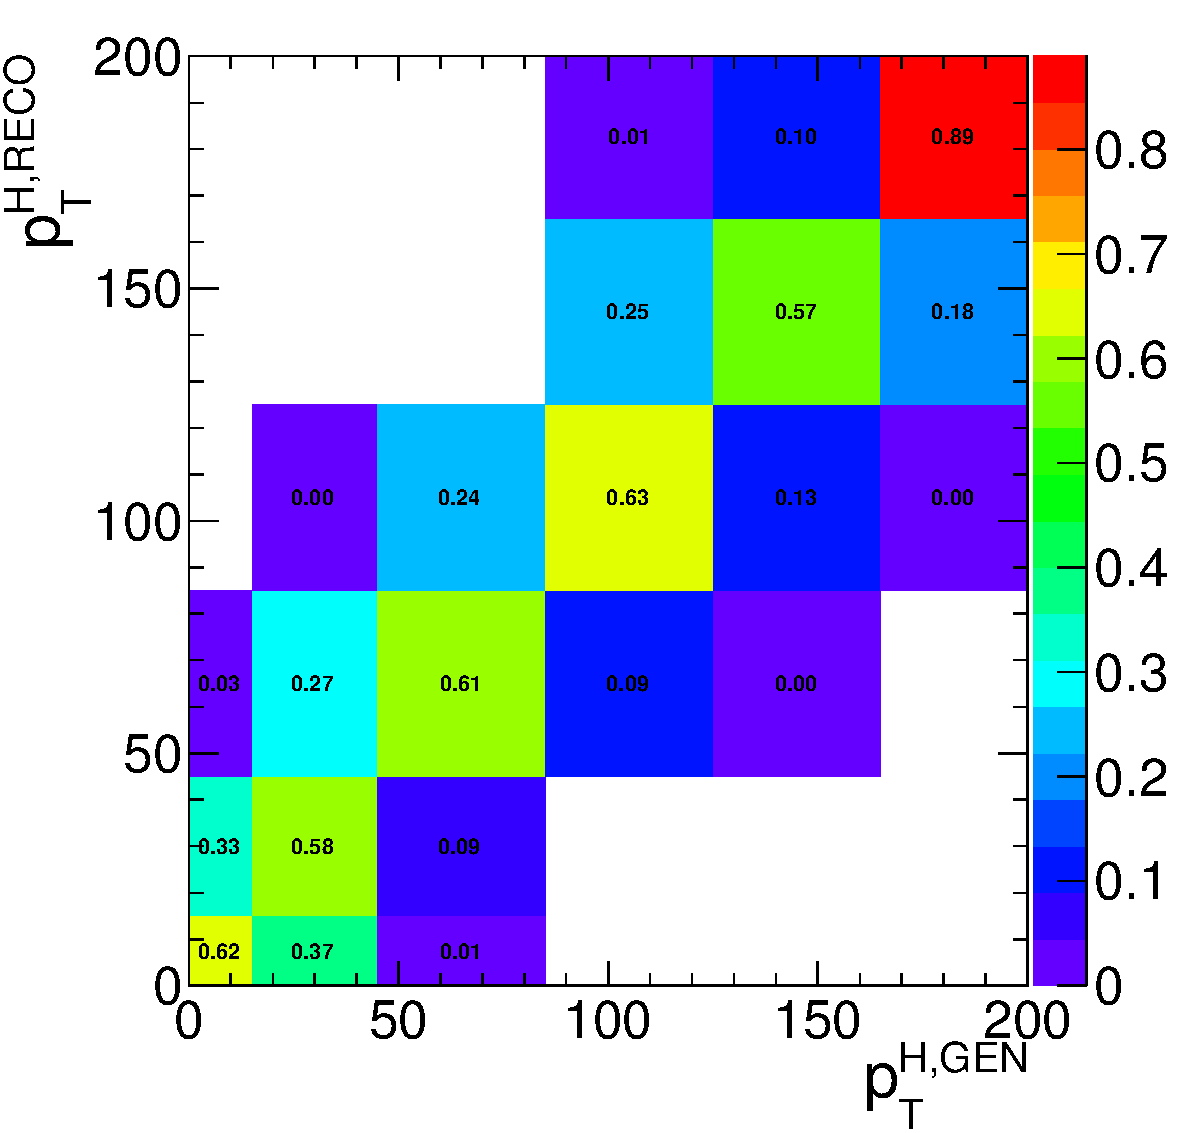
\includegraphics[width=0.45\textwidth]{images/response_ggH_norm_by_row.pdf}}
\subfigure[qqH]{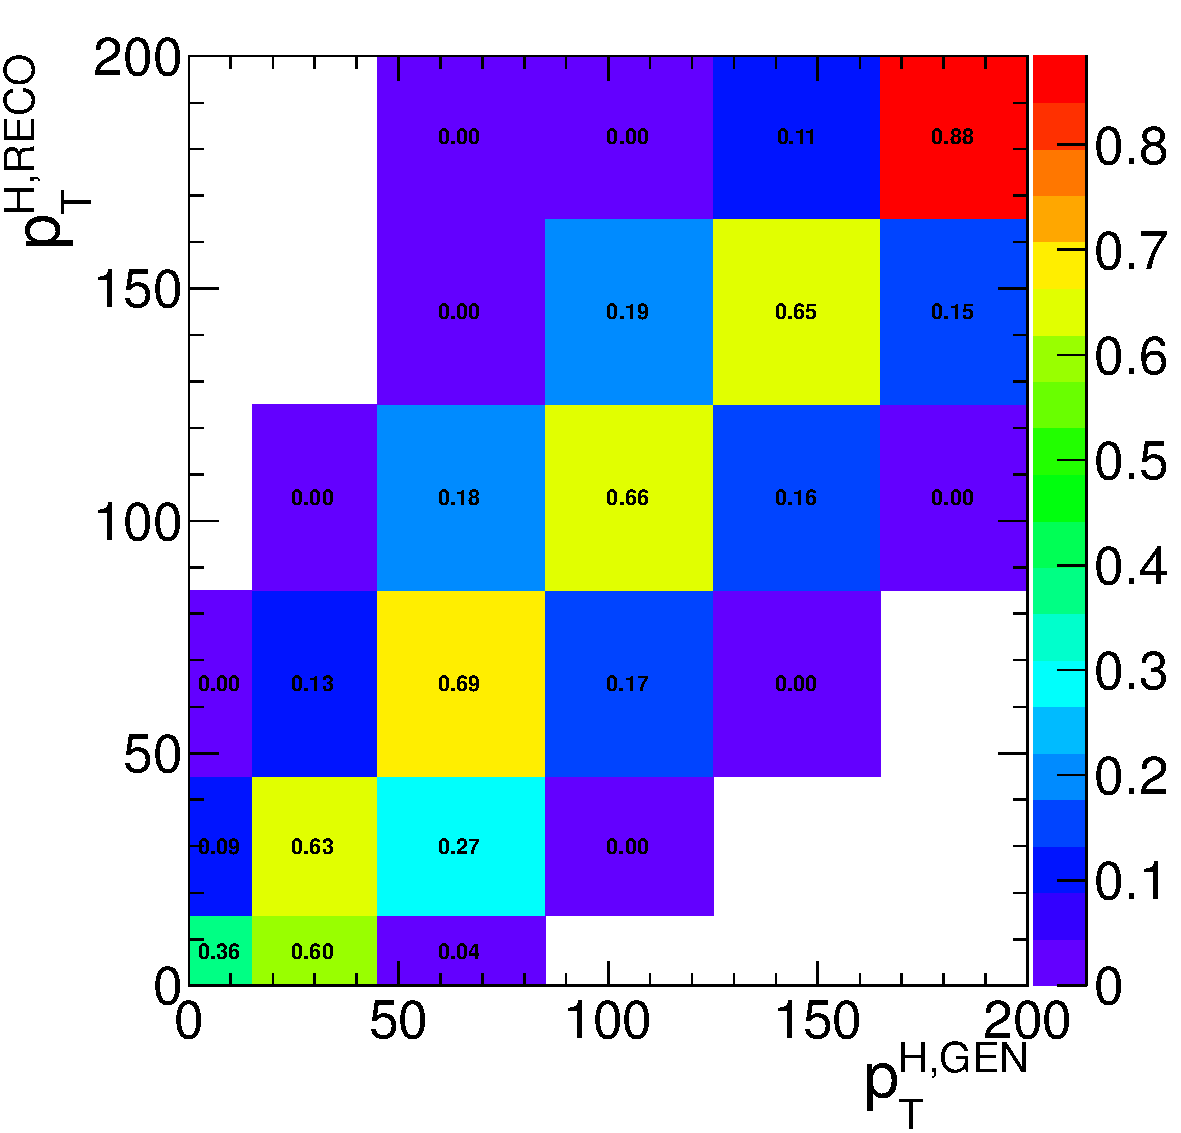
\includegraphics[width=0.45\textwidth]{images/response_qqH_norm_by_row.pdf}}
\caption{Reconstructed versus generated $\pth$ for gluon fusion (a) and VBF (b). Plots are normalized by rows, so that the bin purity is shown on the diagonal.\label{fig:response_by_row}}
\end{figure}
